\documentclass[14pt]{report}
\usepackage{amsmath, amsthm, amssymb}
\usepackage{cmbright}
\usepackage{euler}
\usepackage{setspace}
\usepackage{graphicx}
\usepackage[margin=2.5cm]{geometry}
\usepackage[applemac]{inputenc}
\usepackage[english]{babel}
\setlength{\parindent}{0pt}
\onehalfspace

\begin{document}
\textbf{{Review of Linear Algebra: Questions}}\\
\thispagestyle{empty}


\begin{enumerate}
\item Every plane in $\mathbb{R}^n$ is a subspace of $\mathbb{R}^n$.  

\quad \textbf{TRUE} $\Box$ \quad\textbf{FALSE} $\Box$ 

\item There are $4$ linearly independent vectors in $\mathbb{R}^3$. 

\quad \textbf{TRUE} $\Box$ \quad\textbf{FALSE} $\Box$ 

\item If $Ax=b$ for $A \in \mathbb{R}^{m\times n}$, $x\in\mathbb{R}^n$, and  $b\in\mathbb{R}^m$, then $b$ is a linear combination of the columns of $A$.

 \quad \textbf{TRUE} $\Box$ \quad\textbf{FALSE} $\Box$


\item If $A^2=0$ then A is not invertible.

 \quad \textbf{TRUE} $\Box$ \quad\textbf{FALSE} $\Box$ 



\item The rank $r$ of the $n$ by $n$ matrix $A=[a_{ij}]$ where $a_{ij}=i+j$ is $r=n$.

 \quad \textbf{TRUE} $\Box$ \quad\textbf{FALSE} $\Box$

%\item If $A$ and $B$ have rank $3$ then $A+B$ has rank at most $6$. 

%\quad \textbf{TRUE} $\Box$ \quad\textbf{FALSE} $\Box$ 
 

\item The inverse of an upper triangular matrix is upper triangular. 

\quad \textbf{TRUE} $\Box$ \quad\textbf{FALSE} $\Box$ 

\item For every  matrix $A$ with eigenvectors $v_1, v_2$, the sum $v_1 + v_2$ is an eigenvector of $A$. 

\quad \textbf{TRUE} $\Box$ \quad\textbf{FALSE} $\Box$ 

\item For all $A,B \in \mathbb{R}^{n \times n}$ with $n >1$ it holds that $det(2AB^{-1})=2det(A)det(B^{-1})$. 

\quad \textbf{TRUE} $\Box$ \quad\textbf{FALSE} $\Box$ 

\item For all $A,B \in \mathbb{R}^{n \times n}$ with $n >1$ it holds that $det(A+B)=det(A)+det(B)$.

 \quad \textbf{TRUE} $\Box$ \quad\textbf{FALSE} $\Box$ 


\item Two eigenvectors of a matrix $A$ corresponding to different eigenvalues  are linearly independent.

 \quad \textbf{TRUE} $\Box$ \quad\textbf{FALSE} $\Box$ 

\item A set of vectors that are pairwise orthogonal is 
  linearly independent. 

\quad \textbf{TRUE} $\Box$ \quad\textbf{FALSE} $\Box$ 


\item if $A=[a_{ij}]\in\mathbb{R}^{3\times 3}$, and $E=\left[\begin{array}{ccc}
  1&2&0\\0&3&0\\0&2&1\end{array}\right]$ then the product $EA$ equals...\\

     $\Box$ the matrix formed by adding twice row 2 to each row of $A$.\\
     $\Box$ the matrix formed by adding twice column 2 to each column of $A$. 


\item Let $A\in\mathbb{R}^{m\times n}$ represent a linear transformation
  $\mathcal{A}:\mathcal{V}\mapsto \mathcal{W}$. What is the dimension of $\mathcal{V}$?
What is the dimension of $\mathcal{W}$? Write down the rank-nullity theorem.

% \quad \textbf{TRUE} $\Box$ \quad\textbf{FALSE} $\Box$ \\

\item List all the matrix factorizations that you know.


%\item Let $B$ be the $4\times4$ matrix $B=\left[\begin{array}{cccc}
%  1&5&7&3\\8&9&0&4\\4&2&1&7\\2&3&5&6\end{array}\right]$ to which we apply the following operations:
%        \begin{enumerate}
%          \item[(a)] exchange rows 1 \& 4.
%          \item[(b)] add row 3 to row 2.
%          \item[(c)] exchange rows 1 \& 3.
%          \item[(d)] repplace column 1 by column 4.
%          \item[(e)] delete row 4.  
%        \end{enumerate}
%(i) Write the result as a product of 6 matrices.\\
%(ii) Write the result as a product $ABC$ (same $B$) of three matrices.
  \end{enumerate}
  
%\begin{figure}
%  \begin{center}
%    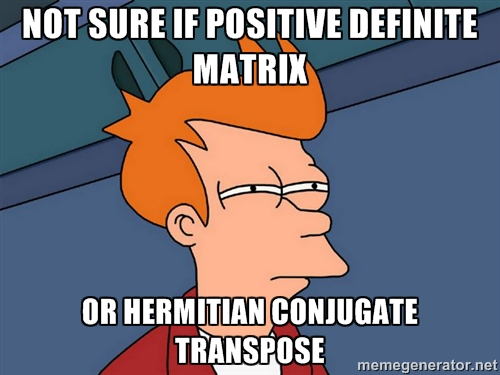
\includegraphics[scale=0.5]{fry2.jpg}\\
%    
\includegraphics[scale=0.13]{chan.png}
%  \end{center}
%\end{figure}

\end{document}
